\chapter{Planificación y Seguimiento}

En este capítulo detallaremos la planificación de cada una de las iteraciones que hemos hecho durante todos los meses de trabajo, así como el seguimiento que hemos realizado de la misma. La elaboración de este proyecto se llevó a cabo durante alrededor de dos años, comenzando en junio del año 2014 y sufriendo un par de interrupciones durante varios meses (desde septiembre de 2014 hasta enero de 2015 y desde mayo de 2015 hasta septiembre del mismo año) a causa de tener que realizar otras actividades que no permitían trabajar en el proyecto al mismo tiempo. También el tiempo dedicado en cada una de las secciones difiere dependiendo del tiempo disponible (durante la mayoría de estos dos años fue necesario compaginer la realización del proyecto proyecto con una jornada laboral a tiempo completo), pero esto es algo que se discutirá en cada una de las secciones individualmente.

Para resumir y clarificar lo que acabamos de comentar, mostramos los periodos de actividad real:

\begin{itemize}
  \item Desde junio del año 2014 hasta septiembre del 2014 (3 meses).
  \item Desde enero de 2015 hasta mayo del mismo año (4 meses).
  \item Desde septiembre del 2015 hasta abril de 2016 (8 meses).
\end{itemize}

\noindent En las próximas secciones hablaremos de lo que hemos desarrollado durante estos tres periodos de tiempo y las iteraciones seguidas en los mismos.

Cabe destacar que todos los datos y tareas mostradas a continuación están realizadas de forma lineal, dado que solamente disponemos de un recurso.

\section{Junio 2014 - Septiembre 2014}

Este periodo comienza el 4 de junio, que es cuando se nos comenta la posibilidad de realizar este proyecto, y termina el 24 de septiembre, por lo que consta de un total de 15 semanas. Hay que tener en cuenta que durante parte de este verano (desde agosto) el proyectando recibe una \textit{internship} en Holanda, por lo que las jornadas de trabajo dedicadas al proyecto solamente constaban de una o dos horas y alrededor de 7/8 horas durante los fines de semana.

Sumando todo el tiempo empleado durante estas semanas se calcula que se han empleado 190 horas en total para la realización de las tareas asignadas a esta iteración en su totalidad.

Durante todas estas semanas el principal objetivo fue el de recoger toda la información general posible para poder empezar el proyecto con buen pie, así como comenzar con la implementación de los mapas y habitaciones que se utilizarán en el juego.

\subsection{Primera iteración: Análisis de requisitos generales, diseño genérico y preparación y configuración de los elementos necesarios para el comienzo de la implementación}

Esta primera iteración empieza el día 4 de junio y termina el 29 del mismo mes. Las tareas realizadas se muestran a continuación:

\paragraph{Análisis de requisitos generales:} Al desarrollar un proyecto enfocado a un sector de la población con necesidades especiales del que no formas parte, es muy importante documentarse sobre todos los aspectos que hay que tener en cuenta e intentar ponerse en su piel (por ejemplo usando las herramientas que ellos utilizan diariamente y así recabar ideas), además de preguntar a diferentes miembros de dichos colectivos para coger distintas perspectivas que luego se puedan incluir en nuestro proyecto.
Asimismo, desarrollar un videojuego puede llegar a ser una tarea sin fin, dado que es común que tanto a desarrolladores como a usuarios se les ocurran continuamente nuevas características o ideas que añadir, y es por eso que debemos sentar las bases que definan lo que es realmente necesario y lo que no para, así, poder priorizar. 
Del mismo modo, aprender sobre lo básico del género y poner límites es fundamental para centrar los reducidos recursos que tenemos en crear lo necesario y luego, si se dispusiese de tiempo, empezar con la implementación de otras características no prioritarias adicionales.

\paragraph{Diseño genérico del juego a implementar:} Crearemos el primer diseño genérico que nos dará una idea sobre lo que tendremos que realizar y nos guiará sobre el proceso de creación del proyecto. Este primer boceto evolucionará a medida que queramos añadir nuevos elementos y ser más específicos en ellos, pero contendrá las partes generales y más básicas de lo que pretendemos realizar.

\paragraph{Búsqueda de bibliotecas que se adapten a nuestros requisitos:} Hay varias bibliotecas con las que se puede crear una interfaz gráfica sencilla como la del videojuego \textit{Rogue} que mencionamos al principio de esta memoria, pero todas ellas tienen sus ventajas e inconvenientes. Debemos averiguar cuáles de ellas son las más adecuadas para nuestro caso y tomar una decisión sobre cuál usar.

\paragraph{Creación y configuración del entorno de desarrollo para poder empezar la implementación:} Al empezar un nuevo proyecto debemos crear un repositorio en \textit{git}, instalar todo el software necesario y preparar el entorno de desarrollo para que podamos empezar a programar sin encontrarnos con ninguna dificultad a posteriori.

\subsubsection{Tareas y seguimiento}

La descomposición de las tareas es la siguiente:

\begin{itemize}
  \item \textbf{WBS 1.1} Análisis de requisitos generales
    \begin{itemize}
      \item \textbf{WBS 1.1.1} Estudio de herramientas para invidentes.
      \item \textbf{WBS 1.1.2} Estudio de los elementos del género \textit{roguelike}.
      \item \textbf{WBS 1.1.3} Analizar los elementos encontrados.
    \end{itemize}
  \item \textbf{WBS 1.2} Diseño genérico del juego a implementar.
  \item \textbf{WBS 1.3} Búsqueda de bibliotecas que se adapten a nuestros requisitos.
  \item \textbf{WBS 1.4} Creación y configuración del entorno de desarrollo para poder empezar la implementación.
\end{itemize}

\noindent Como se puede aprenciar en la Figura ~\ref{fig:sec1it1}, para la realización de todas estas tareas se planificaron 65 horas en total. Esta estimación se cumplió sin ningún imprevisto, por lo que el día 30 de junio todas las tareas habían sido realizadas.

\begin{figure}
    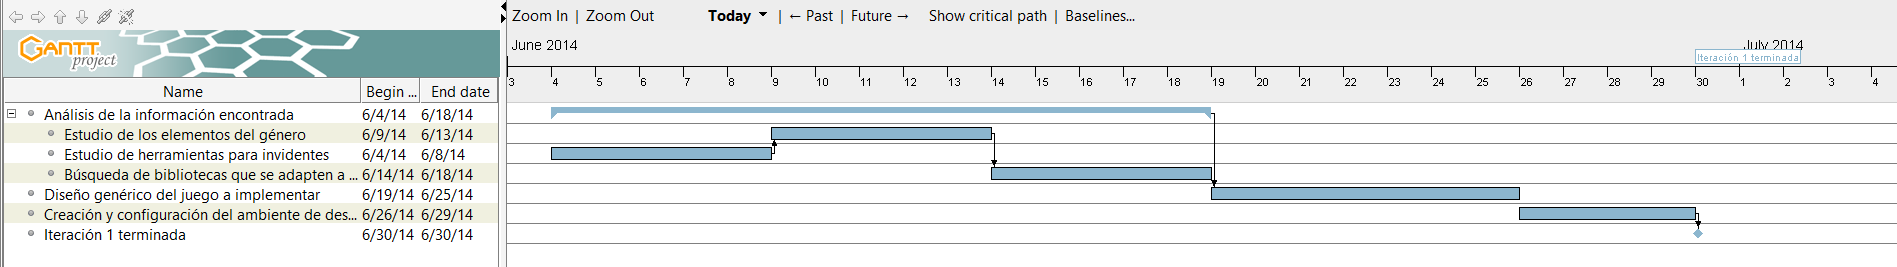
\includegraphics[width=\textwidth,height=\textheight,keepaspectratio]{./img/sec1it1.png}
  \caption{Diagrama de Gantt de la primera iteración de la primera etapa}
  \label{fig:sec1it1}
\end{figure}

\subsubsection{Qué se ha conseguido en esta iteración}

Comenzar un nuevo proyecto e investigar sobre un área que nunca hemos experimentado anteriormente puede ser bastante complicado. En algunas ocasiones la información que nos encontramos puede ser contradictoria o insuficiente, por lo que reconocer lo relevante para nuestro caso es muy importante. Asentar las bases sobre las que se desarrollarán las próximas iteraciones siempre es una tarea ardua y complicada pero necesaria. En esta primera iteración hemos sentado estas bases, definiendo lo que debemos realizar y creando un primer boceto de lo que tendremos que cumplir, concretar, diseñar y programar durante el posterior desarrollo.

\subsubsection{Qué se quiere conseguir en la próxima iteración}

Con todos los aspectos básicos definidos, ahora debemos materializarlos. Durante las siguientes iteraciones deberemos empezar a crear el juego en sí, comenzando por la creación de mapas y habitaciones de manera aleatoria.

\subsection{Segunda iteración: Generación de mapas y habitaciones}

Desarrollada entre el 15 de julio y el 24 de septiembre. Se emplearon 7 semanas para terminar esta iteración, trabajando entre 2 y 3 horas durante los días de semana y alrededor de 7 horas al día durante los fines de semana.

\paragraph{Análisis de requisitos de los mapas y habitaciones:} Hay mucho material escrito y trabajo realizado sobre la creación de mapas y habitaciones de forma aleatoria y pseudo-aleatoria para el género de los \textit{roguelikes}\cite{book:swordscircuitry}. Con toda esta información recogida y recopilada debemos decidir cómo será nuestra solución en base a diferentes factores como, por ejemplo, si el tamaño de dicho mapa siempre será el mismo o no, cómo y cuántas habitaciones queremos tener en cada mapa y el tipo de aleatoriedad a usar (completamente aleatorio o pseudo-aleatorio). Estas decisiones deben concordar con los objetivos que nos hemos marcado anteriormente.

\paragraph{Diseño de los mapas y las habitaciones:} Una vez hayamos creado el análisis de requisitos y tengamos toda la información necesaria sobre la mesa, será hora de crear el diseño. Dicho diseño debe ser fácilmente extensible para que la realización de pequeños cambios no suponga un gran problema.

\paragraph{Creación de tests que cubran lo analizado:} Tal y como comentamos anteriormente a la hora de elegir la metodología en el Apartado \ref{sec:metodologiaelegida}, antes de ponernos con la programación crearemos los tests que especifiquen y cumplan lo diseñado para, posteriormente, proceder con la parte de implementación.

\paragraph{Implementación del diseño de mapas y habitaciones:} Con el diseño y los tests creados, es hora de dar paso a la implementación del código correspondiente. También deberemos de mostrarlo en la interfaz gráfica.

\subsubsection{Tareas y seguimiento}

La descomposición de las tareas es la siguiente:

\begin{itemize}
  \item \textbf{WBS 2.1} Análisis de requisitos correspondiente a la generación de mapas y habitaciones.
    \begin{itemize}
      \item \textbf{WBS 2.1.1} Estudio de diferentes algoritmos de creación aleatoria de mapas y habitaciones.
      \item \textbf{WBS 2.1.2} Decisión sobre la estructura y tamaño a elegir en base al tipo del juego.
    \end{itemize}
  \item \textbf{WBS 2.2} Diseño de los mapas y las habitaciones.
  \item \textbf{WBS 2.3} Creación de tests que cubran lo analizado.
  \item \textbf{WBS 2.4} Implementación del diseño de mapas y habitaciones.
\end{itemize}

\noindent Para la realización de esta segunda iteración se planificaron 125 horas en total, como se puede ver en la Figura ~\ref{fig:sec1it2}, las cuales fueron insuficientes para terminar todas las tareas asignadas inicialmente. Dado que la estimación inicial no fue correcta y no fuimos capaces de finalizar todo lo necesario, tuvimos que dejar la tarea de representar el mapa en la interfaz gráfica para la siguiente iteración.

\begin{figure}
    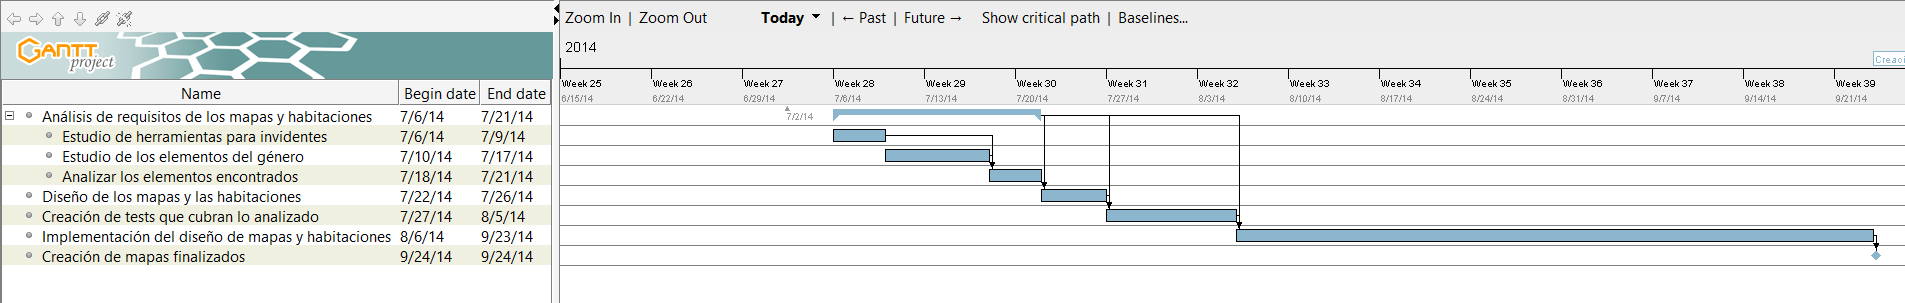
\includegraphics[width=\textwidth,height=\textheight,keepaspectratio]{./img/sec1it2.png}
  \caption{Diagrama de Gantt de la segunda iteración de la primera etapa}
  \label{fig:sec1it2}
\end{figure}

\subsubsection{Qué se ha conseguido en esta iteración}

Hemos conseguido generar mapas y habitaciones de manera aleatoria pero todavía no podemos mostrarlos en la interfaz de usuario. Uno de los puntos esenciales del género de los \textit{roguelike} es su aleatoriedad por lo que conseguir que los mapas puedan ser generados de esta forma es un primer gran hito.

\subsubsection{Qué se quiere conseguir en la próxima iteración}

En la siguiente iteración debemos terminar lo que no hemos conseguido hacer en ésta, por lo que representar estos mapas en la interfaz gráfica toma prioridad. A continuación comenzaremos con la creación de objetos. Dichos objetos son otro de los aspectos esenciales del género y poder generarlos de forma sencilla (al igual que mostrarlos en el mapa) es muy importante, por lo que debemos tenerlo disponible lo antes posible.

\section{Enero 2015 - Mayo 2015}

Este periodo comienza el 2 de enero, tras los festivos navideños, y termina el 31 de mayo, en el que da comienzo el periodo de exámenes. Por lo tanto, esta etapa consta de un total de 21 semanas durante las cuales el proyectando estuvo trabajando a tiempo completo y preparando los exámenes, por lo que el tiempo total semanal empleado en el proyecto se redujo a unas 12 horas de media distribuidas irregularmente. La cantidad de horas dedicadas se analizan con más detalle en cada una de las iteraciones mencionadas a continuación.

En total se dedicaron 170 horas a cumplir todas las tareas que teníamos preparadas para este \textit{sprint}.

En este caso nos hemos centrado en continuar lo realizado anteriormente y, en general, seguir con el desarrollo del juego en sí, centrándonos en los objetos, usuarios, enemigos e interfaz gráfica, dejando para los siguientes \textit{sprints} el tema de las gramáticas para la generación de descripciones.

\subsection{Primera iteración: mapas en IU, análisis, diseño, tests e implementación de los objetos}

Esta primera iteración comienza el 2 de enero y termina el 4 de marzo, por lo que consta de unas 9 semanas en total.

\paragraph{Mostrar los mapas y habitaciones en el interfaz de usuario:} En la anterior fase implementamos los mapas, pero no se mostraban en la interfaz de usuario. En esta ocasión debemos acabar con esta tarea para terminar con todo lo relacionado con la creación de mapas y poder así continuar con el resto de los cometidos que teníamos planeados desde un principio para este \textit{sprint}.

\paragraph{Análisis de requisitos sobre los objetos:} En un \textit{roguelike} los objetos y la interacción con los mismos son primordiales. Debemos estudiar qué objetos vamos a usar y cómo los representaremos en el mapa diseñado en las iteraciones previas.

\paragraph{Crear un diseño simple sobre cómo los objetos interactuarán con el mapa:} Crearemos un diseño genérico que nos permita añadir toda clase de objetos de manera sencilla.

\paragraph{Creación de tests que cubran lo analizado:} Al igual que antes, es necesario crear primero los tests en vez de empezar con la implementación del diseño directamente. En este caso también añadiremos tests en los que interactúen mapas y objetos para asegurarnos que no vamos a tener ningún error cuando combinemos ambos.

\paragraph{Implementación de los objetos en el juego:} Una vez realizado el análisis, el diseño y los tests, podremos implementar la solución encontrada.

\subsubsection{Tareas y seguimiento}

La descomposición de las tareas es la siguiente:

\begin{itemize}
  \item \textbf{WBS 1.1}Mostrar los mapas y habitaciones en el interfaz de usuario.
  \item \textbf{WBS 1.2} Análisis de requisitos sobre los objetos.
    \begin{itemize}
      \item \textbf{WBS 1.2.1} Buscar información sobre los diferentes tipos de objetos necesarios en el juego.
      \item \textbf{WBS 1.2.2} Estudiar cómo estos objetos deben interactuar con el mapa.
      \item \textbf{WBS 1.2.3} Decidir y resumir lo encontrado.
    \end{itemize}
  \item \textbf{WBS 1.3} Crear un diseño simple sobre cómo los objetos interactuarán con el mapa.
  \item \textbf{WBS 1.4} Creación de tests que cubran lo analizado.
  \item \textbf{WBS 1.5} Implementación de los objetos en el juego y su asociación con el propio mapa y habitaciones.
\end{itemize}

\noindent Para la realización de la primera iteración del segundo bloque de trabajo se planificaron 55 horas en total. La estimación fue correcta y fue posible cumplirla, por lo que a principios de marzo tuvimos todas estas tareas terminadas. La Figura ~\ref{fig:sec2it1} muestra información más detallada sobre la distribución de las mismas.

\begin{figure}
    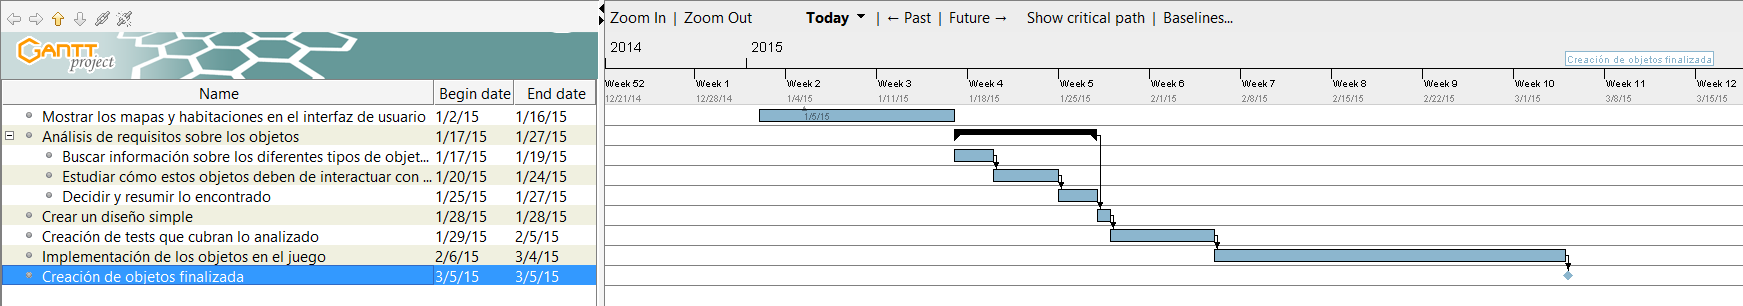
\includegraphics[width=\textwidth,height=\textheight,keepaspectratio]{./img/sec2it1.png}
  \caption{Diagrama de Gantt de la primera iteración de la segunda etapa}
  \label{fig:sec2it1}
\end{figure}

\subsubsection{Qué se ha conseguido en esta iteración}

Terminar la tarea restante que se había dejado inacabada en el \textit{sprint} anterior y permitir la creación y uso de diferentes objetos (pociones, armas y armaduras) con los que los personajes podrán interactuar posteriormente. También ya podemos representar dichos objetos en el mapa y, además, la creación de nuevos elementos resulta muy sencilla gracias al diseño genérico planteado.

\subsubsection{Qué se quiere conseguir en la próxima iteración}

La próxima iteración tendrá que ver con la creación de los personajes. Éste es uno de los pilares esenciales del género y la última pieza que nos falta para tener los elementos primordiales acabados. Por estos motivos es por los que se decidió abordarlo en la siguiente iteración.

\subsection{Segunda iteración: Análisis, diseño, tests e implementación de los personajes}

La segunda iteración comienza el 5 de marzo y acaba el 23 de mayo, contando con un total de 7 semanas de duración. Durante éstas la cantidad de horas trabajadas fue de 11 a la semana.

\paragraph{Análisis de requisitos sobre personajes:} En el juego tendremos un personaje principal, que será controlado por el jugador, y una serie de enemigos con diferentes características que intentarán acabar con él. El jugador deberá enfrentarse a ellos para lograr su objetivo y conseguir mejores objetos que le ayuden a avanzar en el juego. En esta tarea nos encargaremos de buscar información sobre el tipo de enemigos a crear y diferentes métodos para hacerlo de la forma más genérica posible, dado que ser capaz de crear estos enemigos fácilmente es una característica muy importante de nuestro sistema.

\paragraph{Creación del diseño de los personajes:} Una vez hayamos realizado el análisis para hacernos una idea clara de los enemigos y personajes a usar, será hora de crear el diseño. Tal y como hemos comentado en el apartado de análisis, es necesario contar con un diseño fácilmente extendible en el cual aumentar el número de clases generales y tipos concretos de enemigos sea lo más sencillo posible.

\paragraph{Implementación de los tests:} Como hasta ahora, antes de empezar con la implementación directamente, debemos de crear tests sobre ello, que nos indicará las características que deben de cumplir y nos ayudará a detectar fallos en la implementación desde el primer momento.

\paragraph{Programación de lo diseñado y analizado previamente:} Con el análisis, diseño y tests preparados, podremos realizar la tarea de implementación de la creación de personajes y enemigos. Inicialmente solamente contaremos con tres tipos de enemigos a enfretarse, cada uno con características diferentes. Hemos elegido tres tipos de enemigos diferentes porque es suficiente para mostrar la generalidad y aleatoriedad del sistema y nuestro proyecto está más enfocado al procesamiento de lenguages naturales.

\subsubsection{Tareas y seguimiento}

La descomposición de las tareas es la siguiente:

\begin{itemize}
  \item \textbf{WBS 2.1} Análisis de requisitos sobre personajes (jugadores y enemigos)
    \begin{itemize}
      \item \textbf{WBS 2.1.1} Buscar información sobre los diferentes tipos de enemigos a los que nos enfrentaremos.
      \item \textbf{WBS 2.1.2} Estudiar cómo estos enemigos interectuarán con el mapa y los objetos creados anteriormente.
      \item \textbf{WBS 2.1.3} Decidir y resumir lo encontrado.
    \end{itemize}
  \item \textbf{WBS 2.2} Crear un diseño para crear, fácilmente, nuevos enemigos que aparezcan aleatoriamente en el mapa.
  \item \textbf{WBS 2.3} Creación de tests que cubran lo analizado.
  \item \textbf{WBS 2.4} Implementación de los enemigos en el juego y su asociación con el propio mapa, habitaciones y objetos.
\end{itemize}

\noindent Para la realización de todas las tareas de este \textit{sprint} se han asignado 80 horas en total, las cuales fueron suficientes. La Figura ~\ref{fig:sec2it2} muestra información más detallada sobre cómo se han dividido el número de horas por cada una de las tareas.

\begin{figure}
    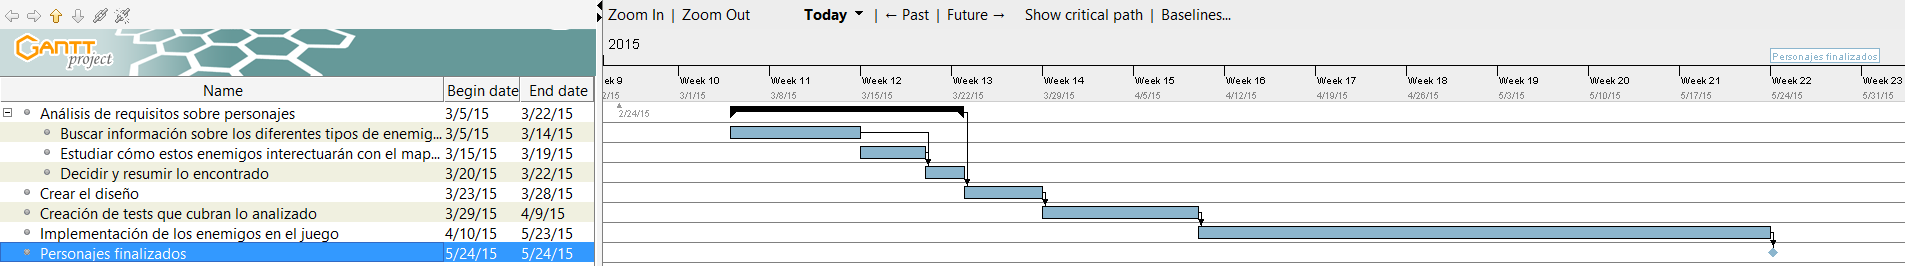
\includegraphics[width=\textwidth,height=\textheight,keepaspectratio]{./img/sec2it2.png}
  \caption{Diagrama de Gantt de la segunda iteración de la segunda etapa}
  \label{fig:sec2it2}
\end{figure}

\subsubsection{Qué se ha conseguido en esta iteración}

Al igual que con los objetos, hemos conseguido facilitar la creación de diferentes tipos de personajes, así como la representación del mapa de los mismos en la interfaz gráfica. 
También hemos creado un personaje principal, que será controlado por el usuario, y diferentes tipos de enemigos a los que enfrentarse: goblins, ratas y dragones. Ambos tipos (el personaje principal y los enemigos) se representan en el mapa de forma diferente para que sea sencilla su identificación.

\subsubsection{Qué se quiere conseguir en la próxima iteración}

Llegados a este punto, el estado del proyecto está bastante avanzado. Al final de este \textit{sprint} tenemos el mapa generado aleatoriamente y en él podemos mostrar objetos y personajes con facilidad, además de que crear nuevos objetos o personajes es ahora algo trivial. El siguiente paso consiste en que los personajes puedan interactuar con los objetos para que así podamos realizar acciones como recoger objetos, equiparlos, tirarlos, etc. También pretendemos que los personajes interactúen entre sí para que, por ejemplo, sea posible que se ataquen entre ellos de diferentes maneras.

\subsection{Tercera iteración: interacción entre personajes, tests e implementación}

Esta última iteración de la sección, y la más corta, comienza el 24 de mayo y acaba el 31 del mismo mes, por lo que su duración es solamente de una semana, aunque al tratase de una semana libre, las horas al día que se pudieran dedicar al proyecto fueron alrededor de seis en lugar de una o dos, que es lo que solíamos trabajar en las iteraciones anteriores.

En la anterior iteración de esta sección teníamos el objetivo de crear los personajes y enemigos y que éstos pudiesen ser representados en la interfaz gráfica. En este caso iremos un paso más allá y añadiremos funcionalidades para que dichos personajes puedan interactuar, comunicarse y usar los objetos presentes en e juego. Para ello crearemos un \textit{inventario} para que el personaje pueda almacenarlos y, de este modo, tanto el jugador como los enemigos puedan tener la habilidad de coger objetos (del mapa al inventario), tirarlos (del inventario al mapa), equiparlos (del inventario al personaje) y desequiparlos (del personaje al inventario). Cuando un personaje muera, los objetos se devolverán al mapa para que puedan volver a recogerse.

\paragraph{Ampliar los tests sobre la interacción entre los objetos y personajes:} En la iteración anterior fuimos capaces de crear los personajes de forma genérica y en este caso deberemos dotarlos con nuevas funcionalidades que ayuden a la interacción entre los objetos y los personajes, tal y como acabamos de describir.

\paragraph{Implementación en base a los tests, análisis y diseño de la anterior iteración:} El diseño y el análisis ya están listos y, una vez tengamos los tests creados, podremos realizar la implementación.

\subsubsection{Tareas y seguimiento}

La descomposición de las tareas es la siguiente:

\begin{itemize}
  \item \textbf{WBS 3.1} Ampliar los tests que tengan que ver con la interacción entre los objetos y personajes.
  \item \textbf{WBS 3.2} Implementación en base al diseño de la anterior iteración y los nuevos tests.
\end{itemize}

\begin{figure}
    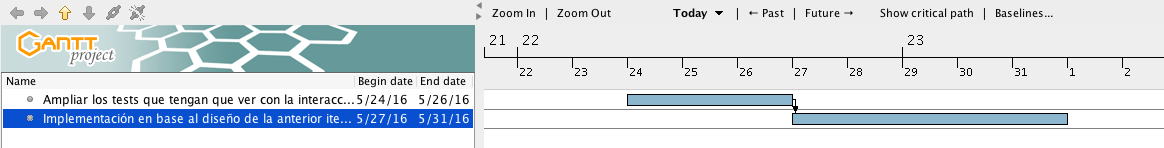
\includegraphics[width=\textwidth,height=\textheight,keepaspectratio]{./img/sec2it3.png}
  \caption{Diagrama de Gantt de la tercera iteración de la segunda etapa}
  \label{fig:sec2it3}
\end{figure}

\noindent Al tratase de un pequeño \textit{sprint} corto y disponer de más tiempo del normal, hemos sido capaces de terminarlo sin mayor problema. El diagrama de Gantt puede verse en la Figura ~\ref{fig:sec2it3} y en él se indica cómo hemos dividido estas dos tareas y cuánto tiempo dedicamos a cada una de ellas.

\subsubsection{Qué se ha conseguido en esta iteración}

En esta iteración hemos conseguido que personajes y objetos interaccionen de una forma básica, lo que constituye un paso previo que nos permitirá, en un futuro, que los personajes utilicen estos objetos para interaccionar entre ellos mismos.

\subsubsection{Qué queremos conseguir en la próxima iteración}

Aumentar esta interacción entre personajes. Por ejemplo, que un usuario pueda ser capaz de atacar a un personaje y que, dependiendo de los objetos equipados, el daño realizado sea mayor. 
También dedicaremos algo de tiempo en dar control al usuario, por lo que tendremos que diseñar la manera de que el usuario pueda decidir moverse, atacar, coger un objeto del mapa, etc. y pensar la manera de distribuir todas estas teclas.

\section{Septiembre 2015 - Abril 2016}

Este periodo empieza el 1 de septiembre, tras un paréntesis en verano, y termina el 31 de abril. Durante esta etapa hemos podido dedicar más tiempo al proyecto que en iteraciones anteriores, alrededor de 20 horas a la semana, con lo que los avances en el proyecto también han sido mucho mayores. Asimismo hemos buscado \textit{feedback} sobre lo que hemos realizado por parte de un grupo de jugadores en potencia y, una vez recibido, las modificaciones y mejoras sugeridas fueron aplicadas durante las últimas iteraciones de este \textit{sprint} asegurarnos para, de este modo, asegurarnos de que es bien aceptado por la comunidad de jugadores invidentes.

Tal y como se puede calcular, este periodo consta de un total de 34 semanas, siendo el periodo más largo de todos los que hemos tenido hasta ahora.

En total, 680 horas fueron dedicadas para este sprint.

\subsection{Primera iteración: Aumentar interacción entre objetos, mapas y personajes, añadir movimiento para el jugador}

Esta primera iteración da comienzo el 1 de septiembre y acaba el 5 de octubre. Su duración total es de 5 semanas.

\paragraph{Aumentar la interacción entre objetos, personajes y mapa:} Hasta el momento tenemos el mapa, objetos y personajes, pero debemos incrementar su capacidad de interactuar (sobre todo entre los personajes, dado que su interacción con los objetos ya se abordó en iteraciones anteriores) así como sus características. Por ejemplo: añadiendo puertas entre habitaciones que también se muestren en el mapa; que el usuario y enemigos puedan atacarse entre sí (teniendo en cuenta las armaduras y armas que llevan); y la integración del concepto ``campo de visión'' para que el personaje del jugador solamente pueda ver lo que hay a su alrededor y no la mazmorra completa.

\paragraph{Agregar \textit{listeners} para que el jugador pueda enviar órdenes al juego} En este momento el jugador aún no puede hacer nada, dado que no hemos creado un sistema para que el usuario pueda moverse o atacar, por tanto, ahora es el momento de introducir los elementos necesarios para que podamos mover nuestro personaje por el mapa y realizar todas las acciones implementadas anteriormente.

\subsubsection{Tareas y seguimiento}

La descomposición de las tareas es la siguiente:

\begin{itemize}
  \item \textbf{WBS 1.1} Aumentar la interacción entre objetos, personajes y mapa.
    \begin{itemize}
      \item \textbf{WBS 1.1.1} Crear tests para los elementos posteriores
      \item \textbf{WBS 1.1.2} Añadir puertas que unan las habitaciones para que el jugador pueda desplazarse de habitación en habitación.
      \item \textbf{WBS 1.1.3} Añadir la posibilidad de ataque entre personajes.
      \item \textbf{WBS 1.1.4} Añadir un campo de visión al personaje del jugador para que no sea capaz de ver todo el mapa, sino el área a su alrededor.
    \end{itemize}
  \item \textbf{WBS 1.2} Agregar \textit{listeners} para que el jugador pueda enviar órdenes al juego.
\end{itemize}

\noindent Hemos estimado 100 horas para este \textit{sprint}, las cuales cumplimos sin problemas. Véase la Figura ~\ref{fig:sec3it1} para comprobar el diagrama de Gantt y obtener información más detallada sobre la división de tareas.

\begin{figure}
    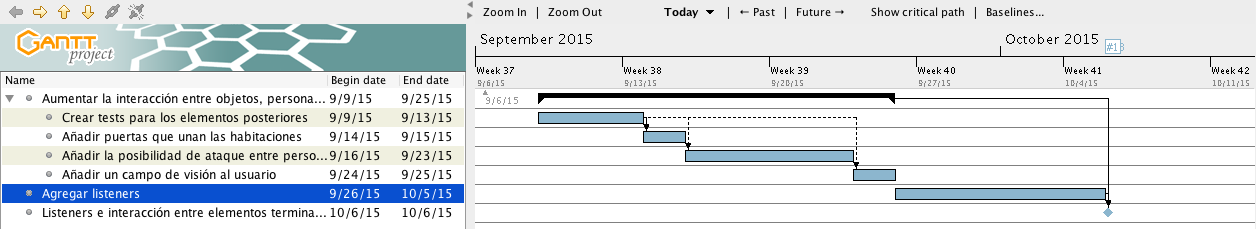
\includegraphics[width=\textwidth,height=\textheight,keepaspectratio]{./img/sec3it1.png}
  \caption{Diagrama de Gantt de la primera iteración de la tercera etapa}
  \label{fig:sec3it1}
\end{figure}

\subsubsection{Qué se ha conseguido en esta iteración}

Al acabar esta iteración contamos con los elementos y funcionalidad básicas de un juego: el usuario puede moverse por el mapa usando el teclado, coger objetos y combatir enemigos (aunque estos enemigos todavía no tienen inteligencia, por lo que no se mueven).

\subsubsection{Qué se quiere conseguir en la próxima iteración}

En la próxima iteración deberemos completar los elementos básicos del videojuego en sí para poder empezar a diseñar la parte de las gramáticas y la generación automática de descripciones. Para ello tendremos que implementar el sistema de portales (que nos permitirán movernos entre mapas consiguiendo, de esta manera, puntos), dotar de una inteligencia artifial (IA) básica a los enemigos e incorporar la opción de cambiar el color de la interfaz de usuario para que se adapte a los jugadores daltónicos, tal y como ya explicamos en la Sección \ref{sec:daltonicossolventar}

\subsection{Segunda iteración: Diseño e implementación de los portales, IA de los enemigos y accesibilidad para daltónicos}

Esta segunda iteración comienza el 6 de octubre y termina el 8 de noviembre, con 4 semanas y media para su completa realización.

\paragraph{Diseño e implementación de los portales:} El sistema de portales fue la idea principal que tuvimos para crear un sistema de puntuación y progreso para el usuario. El objetivo es encontrar el portal dentro del mapa y, una vez localizado, un nuevo mapa será generado, con otro portal en una posición diferente a la anterior. De esta manera, la meta del juego se centra en derrotar enemigos (consiguiendo mejores armas y armaduras en el proceso) para desplazarse de mapa en mapa empleando los portales, y así llegar cada vez más lejos, consiguiendo mejor puntuación.
Deberemos diseñar e implementar estos portales en esta iteración, dado que dotará de un objetivo al título.

\paragraph{Dotar de inteligencia artificial:} Dependiendo del tipo de enemigo al que nos enfrentemos, éste se comportará de forma distinta. Habrá enemigos que serán activos y se lanzan contra el usuario, mientras que otros serán pasivos e inicialmente no querrán atacarlo. Puede ser que en el futuro queramos incrementar la variedad de este tipo de comportamientos. En la Sección \cite{sec:ia} explicamos cómo se ha desarrollado.

\paragraph{Añadir opciones para cambiar el color de la interfaz gráfica:} El punto central de este proyecto es la accesibilidad, e incluir una opción para para mejorar la accesibilidad de los jugadores daltónicos a nuestro juego es muy importante.

\subsubsection{Tareas y seguimiento}

La descomposición de las tareas es la siguiente:

\begin{itemize}
  \item \textbf{2.1} Diseño e implementación de los portales.
    \begin{itemize}
      \item \textbf{2.1.1} Diseñar la mejor manera para incluir los portales en nuestro diseño (en el análisis es algo que se había considerado hacer).
      \item \textbf{2.1.2} Creación de los tests.
      \item \textbf{2.1.3} Implementación de los portales.
    \end{itemize}
  \item \textbf{2.2} Dotar de IA a los enemigos.
  	\begin{itemize}
      \item \textbf{2.2.1} Diseñar la mejor manera para incluir diferentes tipos de IA.
      \item \textbf{2.2.2} Crear los tests de IA.
      \item \textbf{2.2.3} Implementar esta IA para los enemigos.
    \end{itemize}
  \item \textbf{2.3} Añadir opciones para cambiar el color de la interfaz gráfica para usuarios daltónicos
\end{itemize}

\noindent 48 horas fueron las que estimamos suficientes para este \textit{sprint}, resultando suficientes para la conclusión del mismo con todas las tareas terminadas. La Figura ~\ref{fig:sec3it2} proporciona más información sobre la distribución de las tareas mencionadas.

\begin{figure}
    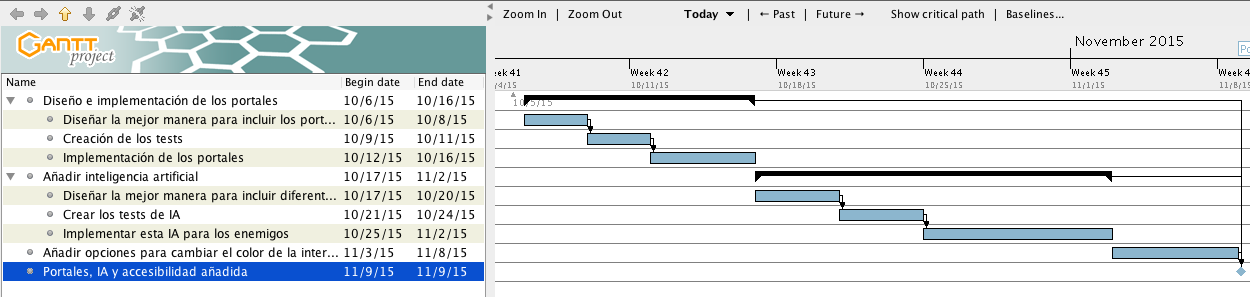
\includegraphics[width=\textwidth,height=\textheight,keepaspectratio]{./img/sec3it2.png}
  \caption{Diagrama de Gantt de la segunda iteración de la tercera etapa}
  \label{fig:sec3it2}
\end{figure}

\subsubsection{Qué se ha conseguido en esta iteración}

Con esta última iteración tenemos la parte básica del juego completada. Hay un objetivo, enemigos con IA que deberemos batir, diferentes objetos que podemos coger, puertas para conectar distintas habitaciones y varias acciones que nos permitirán interactuar con los elementos que acabamos de mencionar.

\subsubsection{Qué se quiere conseguir en la próxima iteración}

Con el juego en sí completado (o por lo menos la parte primordial), es hora de volver nuestra atención a la parte de generación automática del lenguaje y estudiar su integración con lo ya terminado.

\subsection{Tercera iteración: Análisis, diseño básico y comienzo de la implementación de las gramáticas}

Esta segunda iteración comienza el 9 de noviembre y termina el 31 de diciembre, con 6 semanas y media para su finalización.

\paragraph{Análisis de las gramáticas:} Un aspecto clave de nuestro sistema es la generación automática de descripciones de lo que ocurre en el juego para su posterior lectura mediante un lector de pantalla. Buscaremos expresividad y variedad en las descripciones, que se generarán en base a una serie de gramáticas y diccionarios. Esto permitirá, además, traducir nuestro juego a diferentes idiomas de forma relativamente sencilla, pues bastaría con adaptar la gramática y traducir el diccionario empleado. Para construir este motor descriptivo, primero tendremos que investigar cómo podemos hacerlo en nuestro caso de la manera más genérica posible y cómo han solventado este problema otros sistemas similares.

\paragraph{Diseño general sobre la generación del lenguaje:} Una vez hemos analizado y decidido lo que debemos realizar, crearemos un diseño lo más simple y adaptable posible para la generación de dichas frases en base a unas gramáticas del lenguaje dadas. El objetivo principal es, en primer lugar, que la adición de nuevas palabras sea lo más fácil posible para que añadir expresividad y variedad sea sencillo y, en segundo lugar, facilitar al máximo la traducción del juego a otros idiomas.

\paragraph{Creación de gramáticas y diccionarios base:} Para empezar el desarrollo necesitamos tener una gramática y un diccionario base sobre los cuales se comienza a trabajar, analizando los resultados obtenidos. Empezaremos con gramáticas y diccionarios para inglés, dado que sus restricciones iniciales son más sencillas de tratar que en otros idiomas y el número de usuarios potenciales es mayor, aunque mantendremos en mente la futura extensibilidad a otros idiomas con característcias morfológicas que compliquen la implementación (como varios géneros para los sustantivos, artículos, etc.).

\subsubsection{Tareas y seguimiento}

La descomposición de las tareas es la siguiente:

\begin{itemize}
  \item \textbf{3.1} Análisis de las gramáticas.
    \begin{itemize}
      \item \textbf{3.1.1} Familiarizarse con los principios básicos de generación automática de lenguaje.
      \item \textbf{3.1.2} Estudiar cómo construir e integrar un sistema de este tipo en nuestro proyecto en base a lo ya existente.
      \item \textbf{3.1.3} Tomar la decisión en base a lo encontrado y sentar las bases sobre ello.
    \end{itemize}
  \item \textbf{3.2} Diseño general del proceso de la generación del lenguaje y cómo las gramáticas interactuarán con nuestro programa.
  \item \textbf{3.3} Creación de las gramáticas y diccionarios iniciales para tener una base con la que testar nuestra implementación.
\end{itemize}

\noindent Hemos reservado 130 horas para esta iteración y hemos conseguido terminar todas las tareas asignadas a tiempo. En la Figura ~\ref{fig:sec3it3} se puede ver el diagrama de Gantt asociado y obtener más información sobre esta iteración.

\begin{figure}
    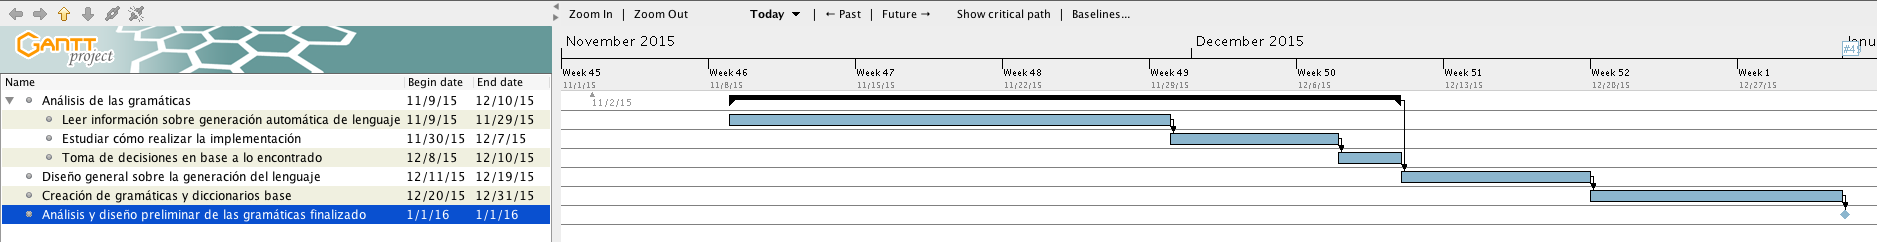
\includegraphics[width=\textwidth,height=\textheight,keepaspectratio]{./img/sec3it3.png}
  \caption{Diagrama de Gantt de la tercera iteración de la tercera etapa}
  \label{fig:sec3it3}
\end{figure}

\subsubsection{Qué se ha conseguido en esta iteración}

Hemos sentado las bases de lo que queremos implementar con las gramáticas en un futuro y hemos creado unas gramáticas y diccionarios iniciales para inglés que iremos ampliando y que servirán de base para el resto de idiomas.

\subsubsection{Qué se quiere conseguir en la próxima iteración}

En la siguiente iteración empezaremos creando los tests para definir cómo las frases automáticas deben generarse e iniciaremos el desarrollo de lo que hemos investigado en esta iteración.

\subsection{Cuarta iteración: Análisis, diseño y comienzo de la implementación de las gramáticas}

Esta segunda iteración comienza el 1 de enero y termina el 14 de enero. Es decir, solamente durará 2 semanas.

\paragraph{Análisis sobre cómo crear las gramáticas NP:} Los sintagmas nominales o frases nominales (NP por \emph{noun phrase}) son elementos básicos de cualquier lengua constituidos, en general, por sustantivos acompañados por sus determinantes (ej. artículos) y modificadores (ej. adjetivos). Sin embargo, su estructura, dada por su gramática, no es igual en todos los idiomas, el orden de los elementos cambia entre inglés y castellano o gallego, por ejemplo. Asimismo debemos estudiar qué planteamientos existen que faciliten su implementación de la forma más genérica posible.

\paragraph{Diseño de las gramáticas NP:} Las frases de sintagma nominal serán las más usadas dentro de nuestro juego. No solamente serán utilizadas al describir lo que sucede en el juego, sino también a la hora de representar los elementos en la interfaz de usuario. Por ello debemos crearlas de la forma más extensible y accesible que podamos.

\paragraph{Creación de los tests para las gramáticas NP:} Al igual que en otras iteraciones, realizamos los tests antes de empezar con ningún tipo de implementación para tener una base sobre cómo las funciones y clases deben de comportase.

\paragraph{Implementación de las gramáticas NP:} Con los tests realizados, debemos empezar con la implementación, teniendo en cuenta el formalismo escogido y las restricciones aplicables en base al idioma. En el caso inicial del inglés, se necesitará abordar el caso de la congruencia en númerp, por ejemplo pero, en su momento, con español también tendremos que tener en cuenta el género.

\subsubsection{Tareas y seguimiento}

La descomposición de las tareas es la siguiente:

\begin{enumerate}[label=\bfseries WBS 4.\arabic*]
  \item Análisis sobre el formalismo a emplear para representar las gramáticas NP y cómo construir un motor de generación de textos descriptivos a partir de ellas para su integración en nuestro sistema, todo ello primando la generidad y la extensibilidad.
  \item Diseño de las gramáticas NP y del motor descriptivo.
  \item Creación de los tests para las gramáticas NP y el motor.
  \item Desarrollo de las gramáticas NP, su enlace con el diccionario e implementación del motor.
\end{enumerate}

\noindent Hemos reservado 40 horas para esta iteración y terminamos todas las tareas a tiempo. En la Figura ~\ref{fig:sec3it4} se puede encontrar más información y para ver el diagrama de Gantt que muestra la distribución de tiempo para estas tareas.

\begin{figure}
    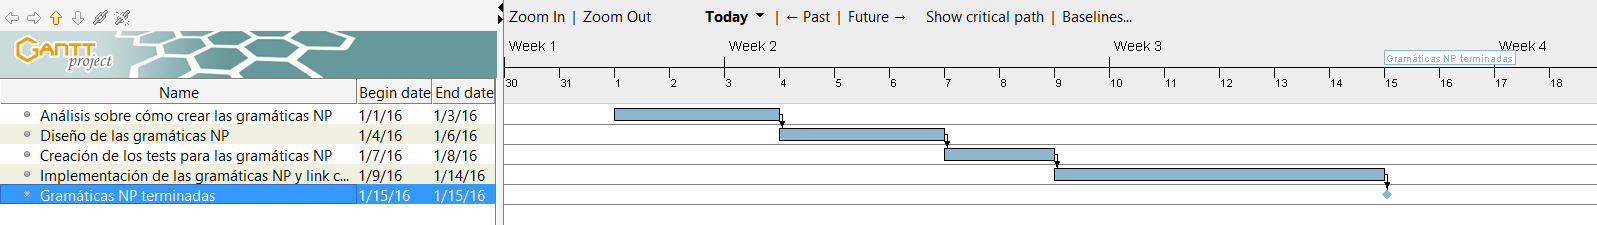
\includegraphics[width=\textwidth,height=\textheight,keepaspectratio]{./img/sec3it4.png}
  \caption{Diagrama de Gantt de la cuarta iteración de la tercera etapa}
  \label{fig:sec3it4}
\end{figure}

\subsubsection{Qué se ha conseguido en esta iteración}

Al finalizar esta iteración hemos conseguido generar sintagmas nominales destinados a describir la acción del juego en base a las gramáticas y diccionarios dados. De momento solamente está disponible para inglés, pero su ampliación a otros idiomas debería resultar sencillo gracias a nuestro diseño y será algo que se realizará en iteraciones posteriores.

\subsubsection{Qué queremos conseguir en la próxima iteración}

Aumentar el rango de las construcciones sintácticas generables a otro tipo de sinftagmas. De esta forma podremos generar diversos tipos de construcciones que permitirán describir todo lo que ocurre dentro de nuestro juego sin problema.

\subsection{Quinta iteración: Análisis, diseño e implementación de las gramáticas y frases más complejas}

Esta quinta iteración comienza el 15 de enero y termina el 29 de enero. Es decir, tiene 2 semanas y media de duración, un poco más que la anterior.

\paragraph{Análisis sobre cómo crear las gramáticas complejas de forma genérica:} Una vez somos capaces de generar sintagmas nominales, pasaremos a combinarlos con otros elementos del lenguaje, tales como verbos para, así, generar estructuras sintácticas más complejas que sean capaces de describir todo lo que realmente deseamos. Deberemos analizar las diferentes formas de hacer esto.

\paragraph{Diseño de dichas gramáticas:} Una vez hayamos analizado y decidido los pasos que vamos a seguir, nos quedará realizar el diseño del mismo.

\paragraph{Creación de los tests para las gramáticas complejas:} Al igual que en las veces anteriores, tendremos que crear los tests antes de empezar con la implementación para estar seguros de que lo que implementamos sea coherente con lo que queremos realizar.

\paragraph{Implementación y enlace con el diccionario:} Desarrollar las nuevas gramáticas más complejas y ampliar el motor de generación acorde con ello para que se comuniquen con las gramáticas NP y nos permitan generar frases y oraciones que describan lo que ocurre en el juego.

\subsubsection{Tareas y seguimiento}

La descomposición de las tareas es la siguiente:

\begin{itemize}
  \item \textbf{WBS 5.1} Análisis sobre cómo crear las gramáticas complejas de forma genérica, extendibles para otros idiomas y que hagan uso de las NP.
  \item \textbf{WBS 5.2} Diseño de dichas gramáticas.
  \item \textbf{WBS 5.3} Creación de los tests para las gramáticas complejas.
  \item \textbf{WBS 5.4} Implementación y enlace con el diccionario.
\end{itemize}

\noindent Hemos reservado 48 horas para esta iteración y la hemos acabado a tiempo. En la Figura ~\ref{fig:sec3it5} se muestra el diagrama de Gantt de esta iteración.

\begin{figure}
    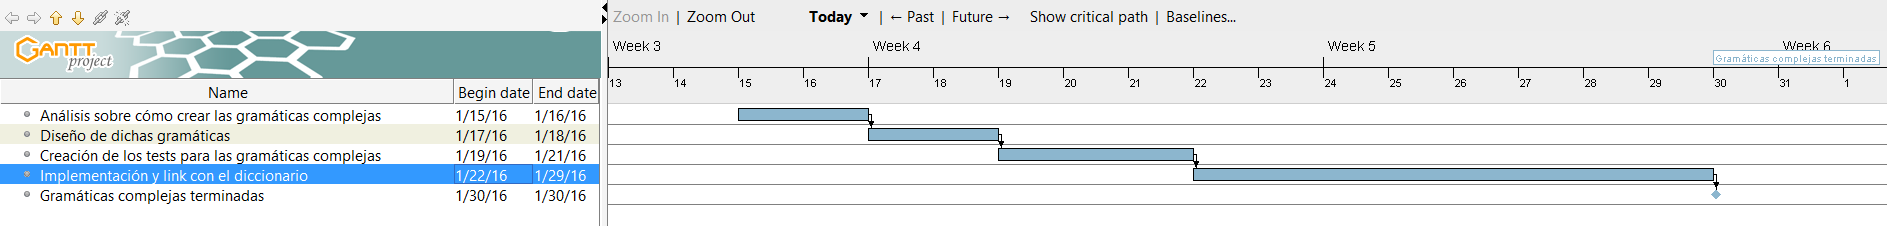
\includegraphics[width=\textwidth,height=\textheight,keepaspectratio]{./img/sec3it5.png}
  \caption{Diagrama de Gantt de la quinta iteración de la tercera etapa}
  \label{fig:sec3it5}
\end{figure}

\subsubsection{Qué se ha conseguido en esta iteración}

Disponer de gramáticas que generen texto para todas las descripciones que contemplamos actualmente en nuestro proyecto. Estas nuevas gramáticas utilizan lo desarrollado en la iteración anterior para, a su vez, formar frases más complejas. También hemos aumentado el tipo de palabras a usar (ahora incluimos verbos y una mayor cantidad de adjetivos y sustantivos), por lo que el diccionario del sistema en inglés, va creciendo. En esta iteración todavía no hemos añadido diccionarios o gramáticas para otros idiomas.

\subsubsection{Qué se quiere conseguir en la próxima iteración}

Las frases y oraciones son generadas, pero todavía no las mostramos en ninguna parte de la interfaz gráfica, por lo que el jugador no puede ni verlas ni escucharlas. En el siguiente \textit{sprint} tenemos que añadir esta opción, además de incluir otros idiomas (es decir, crear las gramáticas y diccionarios correspondientes) como el gallego y español.

\subsection{Sexta iteración: Implementación de las restricciones, gallego y castellano, creación de la interfaz de usuario para con las frases generadas y primer vídeo}

La sexta iteración da comienzo el 30 de enero y terminará el 6 de febrero, por lo que solamente tiene 1 semana de desarrollo, una de las más cortas del todo el proyecto, si bien con una jornada de 8 horas al día en la práctica, por lo que en total fueron 56 horas de trabajo en la misma.

\paragraph{Creación de la interfaz de usuario para mostrar las frases generadas al usuario:} Hasta ahora somos capaces de generar frases que describan lo que sucede en el juego, pero no mostrarlas. Ahora es el momento de mostrar en una ventana la frase generada (de forma similar a un \textit{popup}).

\paragraph{Implementación de las restricciones para el resto de idiomas:} En inglés solamente tenemos que respetar la congruencia en número entre palabras, pero otros idiomas, como el castellano o gallego, tienen otras restricciones adicionales como, por ejemplo, la congruencia en género. Tenemos que tener esto en cuenta e introducirlo en el código.

\paragraph{Añadir gramáticas y diccionarios para gallego y castellano:} La idea desde un principio fue la de extender nuestro sistema la mayor cantidad posible de idiomas, por lo que incluir gallego y castellano es importante. Para ello tendremos que ``traducir'' las gramáticas y diccionarios a ambos idiomas y crear una opción para elegir su uso en un fichero de configuración.

\paragraph{Añadir las teclas necesarias para mostrar las descripciones del inventario y ambiente:} El usuario podrá pedir que se genere una frase que describa algo en concreto. Se debería realizar en base a lo que está especificado en el diagrama de casos de uso.

\paragraph{Crear primer vídeo para recibir \textit{feedback}:} Al terminar esta iteración tendremos el proyecto base completado. Por ello procederemos a grabar un vídeo mostrando el punto en el actual estado de desarollo del sistema con sus funcionalidades y que nos servirá para obtener un primer \textit{feedback} a partir del cual podremos incluir mejoras en futuras iteraciones. A efectos de documentación dicho vídeo aún está disponible en Youtube\footnote{\url{https://www.youtube.com/watch?v=RgND1IGZ-68}}.

\subsubsection{Tareas y seguimiento}

La descomposición de las tareas es la siguiente:

\begin{itemize}
  \item \textbf{WBS 6.1} Creación de la interfaz de usuario para mostrar las descripciones textuales generadas al usuario.
  \item \textbf{WBS 6.2} Añadir las teclas necesarias para mostrar las descripciones del inventario y ambiente, tal y como está definido en el diagrama de casos de uso.
  \item \textbf{WBS 6.3} Integración en el formalismo de las restricciones para el resto de idiomas.
  \item \textbf{WBS 6.4} Añadir gramáticas y diccionarios para gallego y castellano.
  \item \textbf{WBS 6.4} Crear primer vídeo para recibir \textit{feedback}.
\end{itemize}

\noindent En la Figura ~\ref{fig:sec3it6} se muestra el diagrama de Gantt de esta iteración. Hemos reservado, tal y como ya hemos comentado, 56 horas, que fueron suficientes para terminar todas las tareas mencionadas. En dicha figura mostraremos la distribución del tiempo que hemos empleado en cada una de ellas.

\begin{figure}
    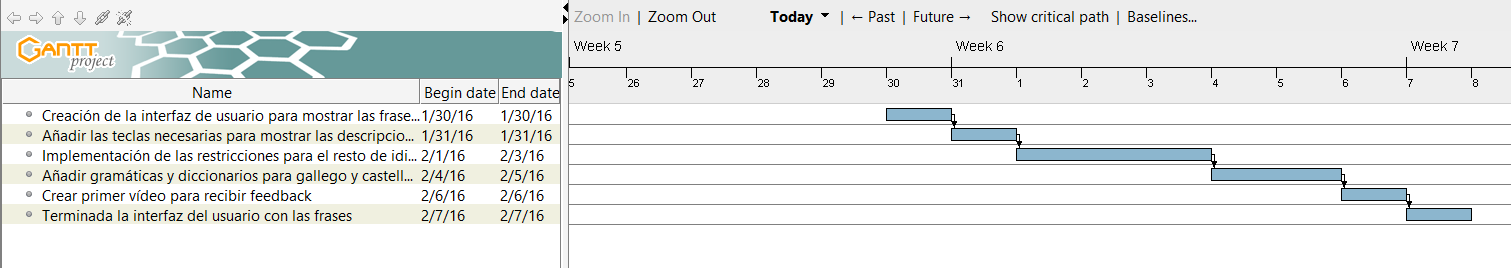
\includegraphics[width=\textwidth,height=\textheight,keepaspectratio]{./img/sec3it6.png}
  \caption{Diagrama de Gantt de la sexta iteración de la tercera etapa}
  \label{fig:sec3it6}
\end{figure}

\subsubsection{Qué se ha conseguido en esta iteración}

Ampliar la cobertura básica del sistema a dos idiomas adicionales (inglés, español y gallego), permitiendo generar las frases necesarias para que el usuario tenga toda la información necesaria y creando un vídeo que nos ayudará a mostrar el funcionamiento del juego a un primer grupo de jugadores (videntes por ahora) para que podamos mejorarlo en base a sus comentarios.

\subsubsection{Qué se quiere conseguir en la próxima iteración}

Debemos esperar por los comentarios y sugerencias recibidos a raíz del visionado del vídeo y, mientras, mejoraremos diferentes aspectos y características del título realizando alguna de las tareas pendientes que tenemos en el \textit{backlog}.

\subsection{Séptima iteración: Resolución de bugs detectados y añadidas pequeñas funcionalidades}

La séptima iteración empieza el 7 de febrero y acaba el 21 de febrero, con una duración de 2 semanas, volviendo a las 20 horas de trabajo por semana dedicadas al proyecto y 40 horas en total para la iteración. Se ha decidido dar un par de semanas de margen para poder leer y recopilar el \textit{feedback} recibido en el marco de la iteración anterior.

\paragraph{Solucionar \textit{bug} en el que la pantalla no se refresca:} En algunas ocasiones y al realizar ciertas acciones, la interfaz gráfica no se actualiza hasta la siguiente acción. Tenemos que solucionar este problema para que lo que se muestre siempre sea lo más nuevo y no haya ningún tipo de retraso.

\paragraph{Cambiar las teclas que usamos por defecto:} Las teclas que tenemos por defecto no son del todo intuitivas. Deberemos cambiarlas para que tengan más sentido.

\paragraph{Definir los adjetivos que describen el estado de los personajes:} Si, por ejemplo, un enemigo tiene poca vida y el personaje que controla el usuario tiene mucha más vida, el sistema reflejará este hecho a nivel descriptivo calificando al enemigo como ``pequeño'', ``insignificante'', etc., mientras que si la situación es al revés, se usará ``grande'' o ``poderoso'', de modo que se verá al enemigo de forma distinta dependiendo del contexto.

\paragraph{Añadir opción para que las descripciones sean cualitativas o cuantitativas:} Cuando escuchamos una descripción, a veces queremos que los contenidos de dicha descripción sean de un carácter más cuantitativo, es decir, que mencione exactamente la vida o posición en coordenadas de los personajes, por ejemplo. Otras veces deseamos que esto no sea así y que todas las descripciones usen expresiones más cualitativas. Crearemos una opción en la que el usuario será capaz de seleccionar lo que prefiera.

\subsubsection{Tareas y seguimiento}

La descomposición de las tareas es la siguiente:

\begin{itemize}
  \item \textbf{7.1} Solucionar bug en el que la pantalla no se refresca cuando es necesario.
  \item \textbf{7.2} Cambiar las teclas que usamos por defecto.
  \item \textbf{7.3} Cambiar los adjetivos que describen los personajes dependiendo de la vida de dichos personajes.
  \item \textbf{7.4} Añadir opción para que las descripciones sean cualitativas o cuantitativas, dependiendo de lo que el usuario desee.
\end{itemize}


\noindent En la Figura ~\ref{fig:sec3it7} se muestra el diagrama de Gantt de esta iteración.

\begin{figure}
    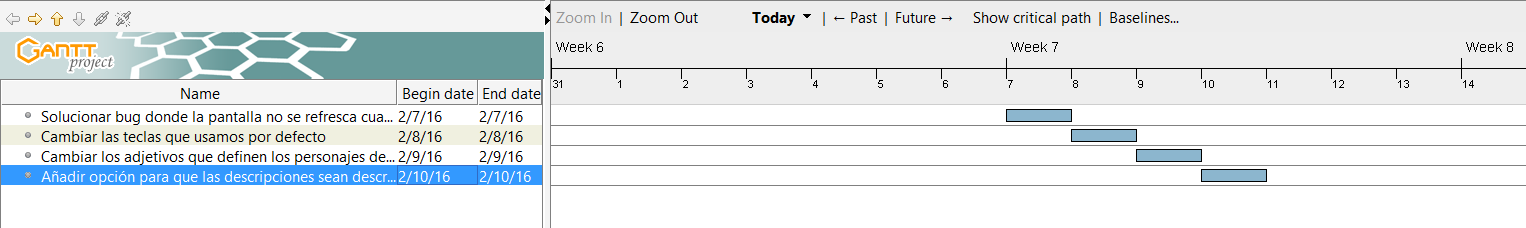
\includegraphics[width=\textwidth,height=\textheight,keepaspectratio]{./img/sec3it7.png}
  \caption{Diagrama de Gantt de la séptima iteración de la tercera etapa}
  \label{fig:sec3it7}
\end{figure}

\subsubsection{Qué se ha conseguido en esta iteración}

Mejorar el juego en diferentes aspectos al añadir nuevas funcionalidades que afectarán directamente al jugador y solucionar algunos de los \textit{bugs} que fueron detectados mientras jugábamos.

\subsubsection{Qué se quiere conseguir en la próxima iteración}

El día 19 de febrero es cuando recibimos el \textit{feedback} que presentamos en la anterior iteración, así que crearemos un \textit{sprint} donde podamos analizar e implementar en su caso los cambios y sugerencias que se nos plantean.

\subsection{Octava iteración: Implementación en base al \textit{feedback} recibido}

En esta iteración nos centraremos en realizar los cambios más importantes, fruto del \textit{feedback} recibido a raíz del vídeo.
Esta iteración contará solamente con 4 días y 20 horas en total, empezando el 22 y acabando el 26, que es cuando publicaremos un nuevo vídeo con los cambios realizados durante las últimas dos iteraciones.

\subsubsection{Feedback recibido}

Todo este \textit{feedback} es el recibido de mano de mis supervisores que, a su vez, se basan en su propio criterio y experiencia y en lo que otros usuarios les han comentado.

\paragraph{Tener en cuenta la persistencia en el tiempo:} Si, por ejemplo, derrotamos a un enemigo, sería una buen adición que las descripciones lo tuvieran en cuenta. De este modo, a la hora de describir de nuevo una sala por la que ya se había pasado y donde se desarrolló un combate, se podría comentar que también se encuentra allí un cadáver.

\paragraph{Cambiar el sistema de salida de las frases generadas:} Hasta ahora, cada vez que una frase era generada, tanto a petición del usuario o en base a una acción que ha sucedido en el juego, mostrábamos una nueva ventana con dicho texto, que tendríamos que cerrar en cada ocasión. Esto es un inconveniente para aquellas personas que sí pueden ver y no quieren ser molestadas por este tipo de ventanas. Tampoco es una solución óptima para los usuarios invidentes, dado que no es lo que se suelen encontrar en otros títulos. La solución que se suele plantear en estos casos es emplear una \textit{textarea}, es decir, una ventana aparte donde se vaya almacenando todas las frases generadas, de tal forma que siempre podemos volver a ella cuando queramos y que, del mismo modo, servirá como un \textit{log} de los sucesos acaecidos durante el juego. En el caso de los jugadores invidentes es importante cambiar el ``foco'' del juego a esta ventana cada vez que una frase sea generada para que el software lector sea capaz de leer lo generado.

\paragraph{Pequeños cambios en los adjetivos usados:} En algunas descripciones el sistema usaba adjetivos poco comunes a la hora de calificar ciertos nombres. Tenemos que cambiarlo para que las expresiones resultantes no resulten extrañas.

\paragraph{Adición de niveles y experiencia:} Los enemigos, armas y el propio usuario deberían tener niveles para que el juego escale en dificultad y aumente en atractivo. Cada vez que se destruye un enemigo, el jugador ganará una serie de puntos que serán usados para subir niveles y, conscientemente, mejorar sus habilidades a la vez que evoluciona el tipo de enemigos a los que se enfrentarán para que la progresión tenga sentido y la experiencia de juego sea gratificante

\paragraph{Cambio en la aleatoriedad:} Hasta ahora, todo lo generado era aleatorio: el tipo de enemigos que nos encontrábamos, los objetos que dejaban atrás éstos al morir, los tesoros etc. Es mejor que esta aleatoriedad venga dada por el nivel del usuario para que el juego escale mejor en dificultad. Esto se explica con mayor profundidad en la Sección: ~\ref{generadorencuentros}.

\paragraph{Mejorar la expresividad:} Algunas de las frases que generamos, por ejemplo, tienden a ser bastante repetitivas o cargantes (``el héroe desequipa la espada'', ``el héroe desequipa la armadura''), en vez de hacer un lenguaje más natural y pulido (``el héroe desequipa la espada y la armadura''). Este tipo de fenómenos han sido tenidos en cuenta.

\paragraph{Darle nombre al héroe:} Siempre nos referimos al personaje que controla el usuario como ``e héroe'' o símplemente ``él'', lo que resulta impersonal. Podríamos darle un nombre o dejar que el usuario elija para dar una mayor variedad y favorecer la empatía con el personaje.

\paragraph{Mostrar estadísticas al cambiar de mazmorra:} Cuando pasamos de una mazmorra a otra usando un portal, podríamos mostrar una serie de estadísticas con los enemigos batidos, la cantidad de experiencia obtenida, el nivel actual del usuario, etc. y, de este modo, dar más sensación de progreso.

\paragraph {Nuevo vídeo} Crearemos otro vídeo integrando los cambios que hemos realizado en base a los comentarios recibidos a raíz del anterior. El vídeo sigue disponible en Youtube.\footnote{\url{https://www.youtube.com/watch?v=3lS0WFrwOeQ}}.

\subsubsection{Tareas y seguimiento}

La descomposición de las tareas que realizaremos este \textit{sprint} es la siguiente:

\begin{itemize}
  \item \textbf{WBS 8.1} Tener en cuenta la persistencia en el tiempo.
  \item \textbf{WBS 8.2} Cambiar el sistema de salida de las frases generadas.
  \item \textbf{WBS 8.3} Pequeños cambios en los adjetivos usados.
  \item \textbf{WBS 8.4} Adición de niveles y experiencia.
  \item \textbf{WBS 8.5} Cambio en la aleatoriedad.
  \item \textbf{WBS 8.6} Mejorar la expresividad.
\end{itemize}

\noindent En la Figura ~\ref{fig:sec3it8} se muestra el diagrama de Gantt de esta iteración.

\begin{figure}
    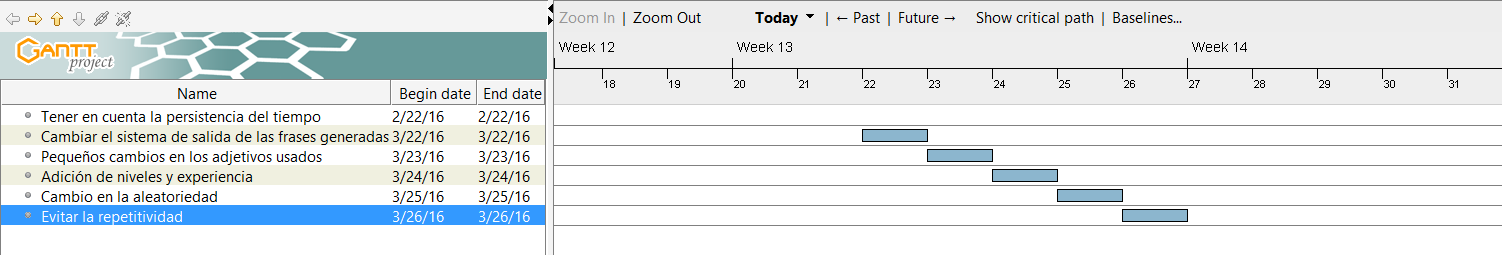
\includegraphics[width=\textwidth,height=\textheight,keepaspectratio]{./img/sec3it8.png}
  \caption{Diagrama de Gantt de la octava iteración de la tercera etapa}
  \label{fig:sec3it8}
\end{figure}

\subsubsection{Qué se ha conseguido en esta iteración}

Hemos conseguido implementar los cambios más importantes en base a los comentarios recibidos, obteniendo así un producto mucho más sólido y adaptado a lo que la comunidad ha considerado más importante.

\subsubsection{Qué se quiere conseguir en la próxima iteración}

En la próxima iteración, que será la última, tendremos que seguir implementando algunas de las tareas que se encuentran en el \textit{backlog} y debemos de tener en cuenta el \textit{feedback} del resto de usuarios, así como el que recibamos de esta iteración.
Las tareas que no vayamos a implementar porque no son completamente necesarias deberán de añadirse al \textit{backlog} para que otros desarrolladores o nosotros mismos podamos tenerlas en cuenta en el futuro.

\subsection{Novena iteración: Más implementación en base al \textit{feedback} recibido}

En esta última iteración daremos los últimos retoques en base al \textit{feedback} recibido de la anterior iteración. Esta última itereación empieza el día 3 de abril, que es cuando recibimos dicho \textit{feedback}, y termina el 13 de abril, fecha que hemos estimado suficiente para terminar las tareas que mencionaremos a continuación. La cantidad de horas usada es la misma que en la anterior iteración, 5 horas al día, por lo que en total trabajaremos 50 horas para finalizar todas las tareas asociadas.

\subsubsection{Feedback recibido}

\paragraph{Añadir el resto de signos de puntuación necesarios:} Algunas de las frases son generadas con los signos de puntuación correspondientes, pero todavía existen partes que no tienen estos signos de puntuación, dando lugar a redacciones extrañas.

\paragraph{Incrementar el tamaño de la fuente dentro del área de texto:} El texto que usamos en la \textit{textarea} no es muy grande, por lo que podría causar problemas a aquellos usuarios videntes con dificultad para leer letras pequeñas. Debemos incrementar el tamaño de la fuente.

\paragraph{Generar todas las frases con las gramáticas:} En el juego tenemos algunas frases que no usan las gramáticas para ser generadas como, por ejemplo, cuando el personaje del jugador muere. Tenemos que cambiar esto para que se adapte al resto del juego y puedan ser fácilmente traducibles.

\paragraph{Cuando pulsemos una tecla en la \textit{textarea}, el resultado debería de afectar el juego:} Cuando pulsamos una tecla para, por ejemplo, desplazar al héroe, mientras el foco está en el área de texto, el foco cambia para el juego, pero la acción correspondiente a la tecla pulsada no es ejecutada. Deberemos solucionar dicho problema.

\paragraph{Cambiar el tamaño y situación de las ventanas:} La interfaz del juego consta de dos ventanas: la primera de ellas corresponde a la interfaz gráfica que muestra el juego en sí, mientras que la segunda es donde se encuentran las descripciones generadas por el sistema. Haremos cambios para que desde el inicio ambas se coloquen y adecúen a la pantalla y no se molesten entre sí.

\paragraph{Añadir sonido cuando el jugador se mueve:} Uno de los consejos que recibimos de la comunidad es el de agregar algún tipo de sonido cuando movemos al personaje, dado que el usuario no recibe ningún tipo de \textit{feedback} de que la acción ha sido realizada.

\paragraph{Refactorizar el código:} Durante el último \textit{sprint} algunos de los módulos contienen código que no es el adecuado. Debemos de refactorizarlo.

\subsubsection{Tareas y seguimiento}

La descomposición de las tareas que realizaremos este \textit{sprint} es la siguiente:

\begin{itemize}
  \item \textbf{WBS 9.1} Añadir el resto de signos de puntuación necesarios.
  \item \textbf{WBS 9.2} Incrementar el tamaño de la fuente dentro del área de texto.
  \item \textbf{WBS 9.3} Generar todas las frases con las gramáticas.
  \item \textbf{WBS 9.4} Cuando pulsemos una tecla en la \textit{textarea}, el resultado debería afectar el juego.
  \item \textbf{WBS 9.5} Cambiar el tamaño y situación de las ventanas.
  \item \textbf{WBS 9.6} Añadir sonido cuando el jugador se mueve.
  \item \textbf{WBS 9.7} Refactorizar el código.
\end{itemize}

\noindent La figura ~\ref{fig:sec3it9} se muestra el diagrama de Gantt de esta iteración.

\begin{figure}
    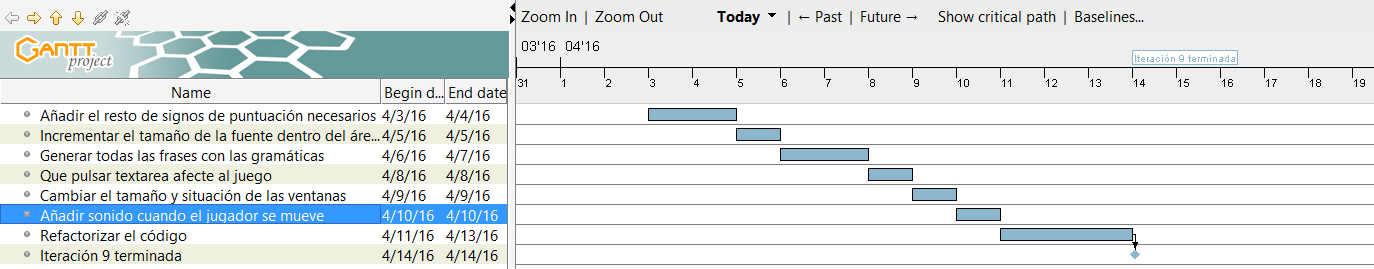
\includegraphics[width=\textwidth,height=\textheight,keepaspectratio]{./img/sec3it9.png}
  \caption{Diagrama de Gantt de la novena iteración de la tercera etapa}
  \label{fig:sec3it9}
\end{figure}

\subsubsection{Qué se ha conseguido en esta iteración}

Terminamos de implementar los puntos más importantes que faltaban o necesitaban revisión, por lo que al final de esta iteración tenemos un juego sólido, extensible y listo para ser jugado y modificado por el resto de la comunidad.

\subsubsection{Qué queremos conseguir en la próxima iteración}
Ésta ha sido la última iteración ``oficial'' del proyecto. En el futuro el juego seguirá evolucionando con nuevas características y aspectos que vendrán dados tanto por nosotros como por la propia comunidad de usuarios, si bien actualmente ha llegado al punto necesario para considerar esta primera versión como finalizada.

Durante el resto de semanas nos dedicaremos a integrar nuevos idiomas (el holandés podría estar disponible en un futuro cercano) e intentaremos buscar miembros de la comunidad que nos puedan ayudar en dicha tarea; dar a conocer nuestro juego a distintas personas y comunidades online para que lo prueben y valores, documentando todo el \textit{feedback} recibido; y crear la documentación del propio título.

\section{Coste del proyecto}

Durante un periodo de trabajo de 15 meses (casi dos años si no contamos los meses sin realizar grandes cambios en la práctica), hemos empleado 1040 horas en la realización del mismo.
El único recurso necesario es el personal, dado que no necesitamos comprar nada de hardware ni ninguna licencia a mayores. Por lo tanto, el coste total del proyecto, suponiendo que el programador trabajara a tiempo completo y cobrará 1200 euros al mes (con una media de 5 euros la hora, contando fines de semana y festivos), sería de 5200 euros.